\section{Proposed methodology}\label{sec:method}

\subsection{Overview}
The routine has three steps (Fig.~\ref{fig:schematic}, Algorithm~\ref{alg:routine}). The \emph{check} uses only the features and labels of the full data set: it predicts how many test rows a random split will place next to a training copy, and how much this can depress coverage for new cases. The \emph{fix} calibrates seen and new rows separately, which restores the promise for new cases whatever the model. The \emph{report} states coverage on new cases next to the usual overall figure. Which parts are standard and which are new is stated with each result.

\begin{figure}[t]
\centering
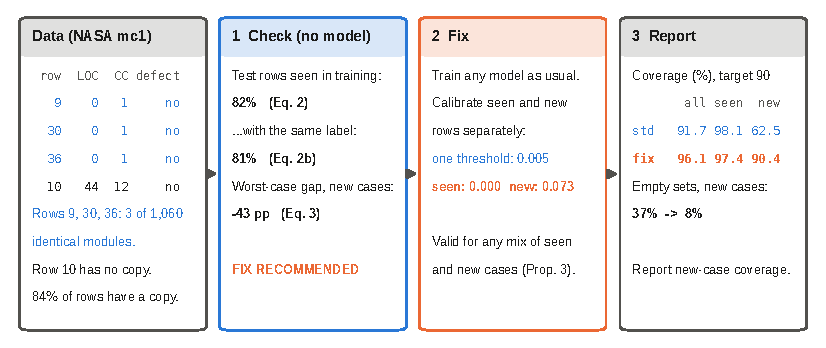
\includegraphics[width=\textwidth]{figures/fig_schematic.pdf}
\caption{The check--fix--report routine, shown with real rows of the NASA mc1 defect data. The check predicts a large shortfall before any model is trained, and the fix restores new-case coverage. The rows shown follow a fixed rule: the first three rows of the largest group of identical modules, and the first row with no copy. All numbers come from the experiment files (random forest, 10 random splits). LOC: lines of code; CC: cyclomatic complexity}\label{fig:schematic}
\end{figure}

\begin{algorithm}[t]
\caption{Check, fix and report conformal coverage for new cases}\label{alg:routine}
\begin{algorithmic}[1]
\Require data $D$, target miscoverage $\alpha$, training share $f$
\Statex \hspace{\algorithmicindent}tolerances $\tau_g=0.02$ and $\tau_\pi=0.10$
\State \textbf{Check} (no model): hash every feature vector; for each row $j$ count its copies $m_j-1$ and the copies with a different label $d_j$
\State compute $\bar\pi$ (Eq.~\ref{eq:exposure}), $\bar\pi_P$ (Eq.~\ref{eq:pure}) and $g^*=-\alpha\bar\pi_P/(1-\bar\pi_P)$ (Eq.~\ref{eq:gstar})
\State \textbf{if} $g^*<-\tau_g$ \textbf{or} $\bar\pi\ge\tau_\pi$ \textbf{then} flag the data set
\State split $D$ at random into $T$, $C$, $E$; fit any model on $T$
\State \textbf{Fix}: label each calibration and test row seen or new by exact match with $T$
\State compute one threshold per group: $\hat q_k=$ the $\lceil (n_k+1)(1-\alpha)\rceil$-th smallest calibration score in group $k$ ($+\infty$ if $n_k<1/\alpha-1$)
\State optionally use the safety-margin rank (Eq.~\ref{eq:pac}) or distance groups instead of seen/new
\State \textbf{Report}: coverage on all, seen and new test rows; for deployment use $\mathcal C(x)=\{y: s(x,y)\le \hat q_{\kappa_T(x)}\}$
\end{algorithmic}
\end{algorithm}

\subsection{Step 1: the check}\label{sec:check}
\paragraph{Exposure.} If a test row belongs to a group of $m_j$ identical rows, and $n_T$ of the other $N-1$ rows go to training, the chance that none of its $m_j-1$ copies lands in training is $\binom{N-m_j}{n_T}/\binom{N-1}{n_T}$. The expected share of seen test rows is therefore
\begin{equation}
\bar\pi=\frac1N\sum_{j=1}^{N}\Big[1-\binom{N-m_j}{n_T}\Big/\binom{N-1}{n_T}\Big].\label{eq:exposure}
\end{equation}
This is elementary combinatorics; \citet{li2026} gives the analogous probability for cross-validation.

\paragraph{Label purity.} Exposure alone can mislead. If repeated rows disagree on the label (identical survey profiles with different outcomes, for example), memorizing them does not help the model. Let $d_j$ be the number of copies of row $j$ whose label (or target value) differs from $y_j$. Row $j$ is \emph{label-pure seen} if at least one copy, but no differently labelled copy, lands in training. Its expected share is
\begin{equation}
\bar\pi_P=\frac1N\sum_{j=1}^{N}\Big[\binom{N-1-d_j}{n_T}-\binom{N-m_j}{n_T}\Big]\Big/\binom{N-1}{n_T}.\label{eq:pure}
\end{equation}

\begin{proposition}[Closed-form label-pure exposure]\label{prop:pure}
Under Assumption~\ref{as:split}, the expected share of test rows that are label-pure seen equals $\bar\pi_P$ in Eq.~(\ref{eq:pure}).
\end{proposition}
The proof is in Sect.~\ref{S-sec:proofs} of the Supplementary Material. On five data sets, the closed form agreed with an average over 30 random splits to within \NPureCfMaxdiff{}.

\paragraph{Predicted shortfall.} Under Assumptions~\ref{as:mem} and~\ref{as:equal}, calibration scores come from a mixture with mass $\pi_P$ at zero and mass $1-\pi_P$ spread by $F$.

\begin{proposition}[Memorization limit]\label{prop:gstar}
Under Assumptions~\ref{as:split}--\ref{as:equal}, as $n_C\to\infty$ the coverage of new cases under standard calibration tends to $1-\alpha/(1-\pi_P)$ for $\pi_P<1-\alpha$, so the coverage gap is
\begin{equation}
g^*=-\frac{\alpha\,\pi_P}{1-\pi_P}.\label{eq:gstar}
\end{equation}
For $\pi_P\ge 1-\alpha$, new cases are almost never covered.
\end{proposition}
We call $g^*$ the \emph{predicted gap}. It is a worst case for models that memorize their training rows. In practice it is computed with $\bar\pi_P$. A data set is flagged if $g^*<-2$ percentage points (pp) or if at least 10\% of test rows are expected to be seen. The second condition guards against failures of Assumption~\ref{as:equal}. This combined rule was written down before either fresh collection was analysed (Sect.~\ref{sec:framework}).

\subsection{Step 2: the fix}\label{sec:fix}
Compute one threshold from the seen calibration rows and one from the new calibration rows, and apply each to the matching test rows. This is Mondrian conformal prediction \citep{vovk2022} with the categories ``seen'' and ``new''.

\begin{proposition}[Validity for any mix; standard]\label{prop:mondrian}
Under Assumption~\ref{as:split}, for $k\in\{\mathrm S,\mathrm N\}$, $\Pr\{Y\in\mathcal C(X)\mid \kappa_T(X)=k\}\ge 1-\alpha$. Coverage therefore holds for any mix of seen and new cases at deployment, including one where every case is new.
\end{proposition}
This follows from the standard Mondrian argument because $\kappa_T$ depends only on the training rows (Sect.~\ref{S-sec:proofs}). If fewer than $1/\alpha-1$ new calibration rows exist, the threshold is $+\infty$ and new cases receive the full set. This is the honest answer when there is no evidence.

\paragraph{Safety margin (standard).} With few new calibration rows, coverage varies from split to split. Using the smallest rank $r$ with
\begin{equation}
\Pr\{\mathrm{Beta}(r,n-r+1)<1-\alpha\}\le\delta\label{eq:pac}
\end{equation}
gives coverage of at least $1-\alpha$ with probability at least $1-\delta$ over the calibration draw \citep{vovk2012}. We use $\delta=0.1$.

\paragraph{Calibration by distance.} Exact matching cannot see near-copies. As a variant, calibration and test rows are grouped by the distance to their nearest training row: exact copies form one group, and new rows form five groups at training-only distance quantiles. Each group is then calibrated separately, as in difficulty-based Mondrian calibration \citep{bostrom2020}.

\subsection{Step 3: the report}
Report coverage on new cases, the share of seen test rows, and the set size for new cases next to the usual overall coverage. A reader can then judge the evaluation without rerunning it.

\subsection{The \emph{covercheck} tool}\label{sec:tool}
We packaged the routine as an open-source Python library and command-line tool. \texttt{check(X, y)} computes Eqs.~(\ref{eq:exposure})--(\ref{eq:gstar}) and returns a verdict with reasons. \texttt{SeenNewConformal} wraps any scikit-learn estimator and implements the fix, the safety margin and the distance variant. \texttt{evaluate} reports coverage on all, seen and new cases over repeated random splits. The command \texttt{covercheck data.csv --target label --html report.html} runs all three steps. The tool has its own test suite, which includes a simulation check of Eq.~(\ref{eq:pure}) and of the fix.
